\documentclass{article}
 
\usepackage[margin=1in]{geometry}
\usepackage[strict]{changepage}
\usepackage{float}
\usepackage{fancyhdr}
\usepackage{mhchem}
\usepackage{siunitx}
\usepackage{wrapfig, booktabs}
\usepackage{enumitem}
\usepackage{ctex}
\usepackage{graphicx}
\usepackage{amsmath}
\usepackage{bbding}     % for checkmark 
\usepackage{pifont}     % for checkmark 
\usepackage{wasysym}    % for checkmark 
\usepackage{amssymb}    % for checkmark 
\usepackage{subfigure}
\usepackage{multirow}
\usepackage{multicol}
\usepackage{wrapfig}
\usepackage{indentfirst}
\usepackage[utf8]{inputenc}
\usepackage{geometry}
\usepackage{setspace}   %set space between lines
\usepackage{graphicx} %insert figure 
\usepackage{float} %设置图片浮动位置的宏包
\usepackage{subfigure} %插入多图时用子图显示的宏包
\usepackage{listings}   %插入代码的宏包
\usepackage{xcolor} % to define color 
\usepackage{verbatim}   %for comment 
\usepackage[breaklinks,colorlinks,linkcolor=black,citecolor=black,urlcolor=black]{hyperref} %for bookmark 

\setlength{\parindent}{2em}

\definecolor{mygray}{rgb}{0.5,0.5,0.5}  %totally used in code display
\definecolor{mygreen}{rgb}{0,0.6,0}

\lstset{                %代码显示格式设置
    numbers=left,                                   
    % where to put the line-numbers; possible values are (none, left, right)
    numberstyle=  \color{mygray}, 
    % the style that is used for the line-numbers
    keywordstyle= \color{ blue!70},
    basicstyle=\footnotesize,        
    % the size of the fonts that are used for the code
    commentstyle=\color{mygreen},    
    % comment style
    frame=single,	                   
    % adds a frame around the code, you can use frame=shadowboxs
    % with a rulesepcolor= \color{ red!20!green!20!blue!20} ,
    escapeinside=``, % 英文分号中可写入中文
    xleftmargin=4em,xrightmargin=2em, aboveskip=1em,
    framexleftmargin=2em
} 


\begin{document}

\begin{spacing}{1.5}

    %title  page 
    \thispagestyle{empty}
    \begin{center}
~\\[6cm]\rule{\linewidth}{0.5mm} \\[6mm]
{\Large 电子设计  \\  \textbf{{\LARGE 预习报告}}  \\[6mm]}
\rule{\linewidth}{0.5mm} \\[2cm]
{\Large 姓 名: 吕光冉}\\[.3cm]
{\Large 班 级:   自73 }\\[.3cm]
{\Large 学 号:  2017011574}\\[.3cm]
{\Large 日 期:\today }\\[.3cm]
    \end{center}

    \clearpage
    \phantom{s}

    %if need to make table of contents in pdf, below command is okay
     \tableofcontents
     \newpage

    %section 1: aim
\section{选题背景}

    \subsection{眼动追踪技术}
 
从历史上看,每一次人机交互方式的变化都必然会带来一场科技的革命。上世纪80年代,鼠标与图形桌面的发明使得电脑开始步入PC时代。90年代触摸屏的出现,直接为新一代智能手机和平板的问世奠定了基础。现在,随着物联网的普及和5G时代的到来,我们需要交互的电子设备的数量也将与日俱增。而眼动追踪技术的发展,则给新时代人机交互的方式创造了无限可能。

​眼动追踪技术多是依赖于眼动仪来实现。眼动仪指的是一种能够跟踪测量眼球位置及眼球运动信息的设备,它能够测量人眼注视点以及眼球相对头部的运动轨迹。其原理为:使用人肉眼不可见的红外光对人眼进行照射,然后对反射回来的红外线进行成像。由于瞳孔不可反射红外光的特性,整个红外成像图中仅有瞳孔处为纯黑色,这就为瞳孔的识别奠定了基础。

​尽管眼动追踪技术在近年来才开始进入大众的视野,实际上其历史悠远流长。早在上世纪三十年代,第一台非侵入式的眼动追踪就已经问世。但是初期的眼动追踪仪不仅体积过大,
使用不方便,还存在计算量过大,算力要求高的问题。这一时期的眼动追踪设备多数仅能放置在实验室中。但近年来,随着计算机性能的不断提高与计算机视觉和人工智能技术的不断发展,眼动追踪技术的实现对于体积和算力的要求大大降低,越来越多的个人用户开始享受到眼动追踪技术所能带来的乐趣。

​在现在,眼动追踪这一技术开始有越来越多的应用。除了比较常见的心理学测试以及残疾人辅助的用途,眼动追踪还有着市场研究与消费者调研,人机交互,人的效能研究等多种应用。而本项目将根据眼动追踪技术所获得的眼动信息进行机器人控制,从本质上来说也属于人机交互的一种。


    \subsection{视觉识别}

视觉识别是机器视觉的一个分支,指的是依赖于相机、摄像头等传感器,配合机器视觉算法进行物体识别。这一分支的发展历史十分悠久,早在上世纪80年代就已经出现。而由于最近深度学习这一革命性技术的发展,视觉识别开始进入普通大众的视野。

视觉识别的实现方式主要分为传统视觉方法和深度学习两种。在拥有大量数据集时,一般深度学习方法给出的识别准确度要比传统视觉方法高很多。但是当数据集较小,甚至没有数据集时,传统视觉方法通常优于深度学习。
    
在本项目中,将要实现的识别任务主要包括三个:人体识别,障碍识别,以及小车识别。其中,人体识别和障碍识别都有大量的数据集,可以使用深度学习的方法实现。但是小车由于其形状比较特殊,与普通车辆并不相同,所以可能深度学习所得识别效果并不能满足需求。这时可以考虑使用传统视觉方法中的色块识别,二维码识别,以及小车的模式匹配等方式来解决问题。
    
    \subsection{跟踪机器人}

基于机器视觉来实现跟踪机器人是近几年的世界各地开发者和研究人员的一个热点话题$^{[1][2]}$。在开发者们的设计方案中,视觉来源包括外部摄像头,机器人上的机载摄像头等,使用的视觉方法包括传统视觉和深度学习,实现的硬件平台有多轮小车,足式机器人和无人机等,而硬件控制手段包括有普通代码 ,ros 甚至是 PLC 的方式。

​在本项目中,由于机器人控制并不是本项目的开发重点,所以会使用轮式机器人加 python 脚本的方式简化机器人控制端。同时,在机器视觉的基础上,融入眼动追踪技术来帮助机器人进行更加智能的决策。
    %section 2: prepare 
\section{项目设想}

​	本项目将实现一个能够自主跟踪人类,并在人类注视它时自动停下,甚至小幅度后退的跟踪机器人。具体来说,其功能包括:

    \begin{enumerate}
        \item 能够识别人体并自动跟随
        \item 实现一定的避障功能
        \item 在人注视时,能够停下并小幅度后退(这时由于没有后视摄像头,所以不要求具备后向避障功能)。
    \end{enumerate}

\section{初步方案}

    \subsection{硬件设计}

本项目设计的硬件系统框图如图\ref{fig:hardware}所示:

\begin{figure}[H]
    \centering
    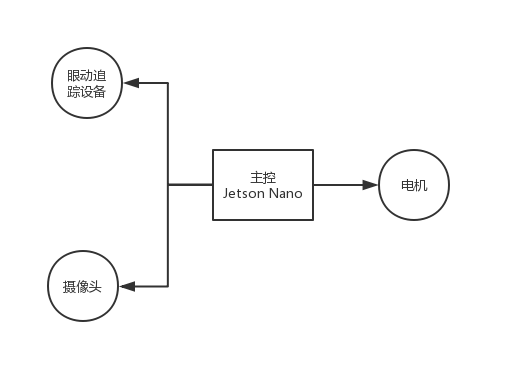
\includegraphics[scale=0.4]{fig/hardware.png}
    \caption{硬件系统}
    \label{fig:hardware}
\end{figure}


其中,本项目使用 Nvidia (英伟达)公司于今年3月最新发布的 Jetson Nano 作为主控板。

\begin{itemize}
    \item 上面载有四核 Cortex-A57 处理器(CPU),128个 Nvidia CUDA 核心的 NVIDIA Maxwell 架构显卡,4GB内存, 128G tf 卡式存储。其计算性能最高能达到 472 GFLOPS,耗电功率仅为 5W。并且它支持 Jupyter Notebook 在线开发,简化了调试和运行的流程,提升开发速度$^[3]$。
\end{itemize}

使用 Jetson Nano,归功于其强大的计算能力,可以在上面运行小型神经网络(选择使用 SSD 神经网络)。通过其与摄像头,电机的配合,可以实现人体识别、跟随、以及避障的功能。

本设计的传感器包括眼动追踪设备和车载摄像头两个。

\begin{itemize}
    \item 眼动追踪设备使用的是由 VUELOSOPHY 提供的眼动开发套件。其基本原理与在眼动追踪章节处叙述的相同。它支持网络开发,可以在同一局域网内以 json 格式获取眼动数据。通过其与Jetson Nano 主控板的配合来实现眼动数据的获取和分析。
    \item 摄像头使用的是 RPi Camera V2 这款树莓派原生鱼眼摄像头,其分辨率最高可达300x300,能够满足项目的基本需求。
\end{itemize}

本设计的执行机构只有两个电机,以及对应的 pwm 两路驱动模块。由于结构简单,在此并不详细叙述

而整个系统所使用的电源为:
\begin{itemize}
    \item 5V 20000mAh 的小米充电宝。由于系统整体功耗较低(主要耗电元件中,主控板功耗低于5W,两路电机功耗低于8W),且都支持 USB 供电,所以电池容量为 20000 mAh,瞬时功率输出最高可达 18W的小米充电宝是满足系统的供电需求的。
\end{itemize}


    \subsection{数据流设计}

    本项目设计的数据流分析如图\ref{fig:data_flow}所示:
\begin{figure}[H]
    \centering
    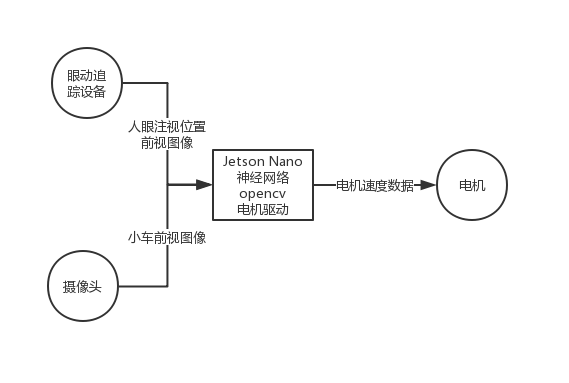
\includegraphics[scale=0.4]{fig/data_flow.png}
    \caption{数据流框图}
    \label{fig:data_flow}
\end{figure}

本设计中,传感器数据包括有:
\begin{itemize}
    \item 人眼注视位置(来自眼动追踪设备, json 格式)
    \item 眼镜前视图像(来自眼动追踪设备, json 格式)
    \item 小车的前视图像(来自车载摄像头,numpy 格式)
\end{itemize}

在Jetson Nano上,通过使用预先训练好的神经网络,对车载摄像头给出的前视图像进行分析,可以完成障碍和人体的识别任务。而对于眼镜的前视图像,可以使用传统视觉(基于 opencv实现)或者深度学习的方式,分辨出视觉范围内的小车位置,再与眼镜所传出的人眼注视位置相比较,判定人是否在注视小车。

也就是说,经过数据处理后,获得的信息包括以下几个方面:
\begin{itemize}
    \item 人体位置 (来自车载摄像头,只需判断中心点在画面的左边,右边,中间)
    \item 障碍位置(来自车载摄像头,二值数据,判断前方是否有障碍)
    \item 小车位置(来自眼镜前视摄像头,只需要和人眼注视位置进行比较)
    \item 是否在注视小车(来自眼镜前视摄像头,二值数据,判断是否正在注视)
\end{itemize}

根据以上信息,由小车自主进行决策。其需要控制的执行机构有:

\begin{itemize}
    \item 左右两路电机(pwm波控制,由电机驱动进行辅助控制,通过两路速度的控制完成前后左右的移动)
\end{itemize}

整个系统的供电由于没有数据流信息,所以在此并不详细叙述。

\subsection{任务清单}

根据初步的项目方案,所需要完成的任务清单如下:

\begin{itemize}
    \item 小车跟踪和避障功能的实现。其中子任务包括:

    \begin{itemize}
        \item 小车硬件的制作。包括车轮、电机、电机驱动的选购,车身框架的制作。对于车身框架,可以使用 GitHub 上的开源项目 Jetbot 所提供的文件来实现。
        \item 车载主控板 Jetson Nano 的调试。包括有系统镜像安装,软件环境配置等。但是 Nvidia 公司官方提供现成的镜像文件,所以也并不复杂。
        \item 神经网络的训练和提交。我所使用的为 Pytorch 框架下的 SSD 网络。网络架构和节点数据都使用预训练数据,视检测情况判断自己是否需要自行制作数据集并进一步训练。
        \item 整体检测与控制。在确保可以实现障碍和人体检测的视觉检测功能后,将其作为决策的基础,使其能够自行避障并跟随人移动。
    \end{itemize}

    \item 眼动追踪眼镜的调试与信息获取。其中子任务包括:
    \begin{itemize}
        \item 眼动追踪眼镜 API 的使用。由于其编程主要都是基于网络编程,所以需要自己发命令并接受相应数据,并对数据进行相应处理。由于其数据使用的都是 Json 格式,所以利用 Python 中的 Json 包可以解析相关数据。
        \item 对图像进行处理,识别小车。这一点是眼动追踪眼镜开发中最为困难的一步。其最简单的替代实现方式是让小车车载二维码或者色块,再加上Opencv进行小车识别。最困难的实现方式为使用传统视觉或者深度学习的方式来实现,但是这两个实现方式都可能会遇到数据集不足和特征不明显的问题。
    \end{itemize}

    \item 综合调试,即将前两部分中所获取到的信息进行整合,最终写一个整体的控制程序。其中子任务包括:
    \begin{itemize}
        \item 在前两步中查看使用的计算资源的情况,判断在这一步中是否会出现资源不够的问题。如果出现,可能需要将一部分图像处理任务交给上位机进行实现,然后通过 wifi 将处理结果交给主控板。
        \item 解决运行逻辑冲突问题。可以会使用中断或者多线程同时处理的方式来提升程序的实时性。
    \end{itemize}
\end{itemize}

\section{创新点}

本项目的主要创新点包括:

\begin{enumerate}
    \item 设计创新。本项目从项目设计上来说,在实现基础的跟踪和避障功能的基础上,还实现了反跟踪的功能,具有一定程度的人机交互的特点。
    \item 手段创新。本项目中,控制机构使用了 Nvidia 最新推出的 Jetson Nano 开发板。可以在开发的同时,体验新版 Jetson 开发板的开发特点,并与之前使用过的 Jetson TX2 进行性能和开发难易度比较。
    \item 信息来源创新。在本项目中,利用眼动追踪设备,使用眼动信息和前视图像来共同决策机器人的运动。
    \item 数据传输手段创新。在本项目中,所有设备(包括上位机,Jetson Nano,眼动追踪所使用到的树莓派)之间的数据传输,都是基于 wifi 来进行传输。这样一来避免了相互之间的物理连线,方便用户使用和调试。
    \item 可扩展。本项目中实现的仅为跟踪和反跟踪的基本原理。可以在本项目的基础上,更换硬件平台为其他具有更多自由度的机器人,硬件控制可以使用更加强大的 ROS 开源系统,眼动跟踪设备可以改用为车载的遥感式眼动跟踪设备,不再需要人体佩戴眼动追踪眼镜。
\end{enumerate}

\section{现有成果}

按照任务清单,其中已经完成的任务包括:

\begin{itemize}
    \item \CheckedBox 小车跟踪和避障功能的实现。其中子任务包括:

    \begin{itemize}
        \item \CheckedBox 小车硬件的制作。包括车轮、电机、电机驱动的选购,车身框架的制作。对于车身框架,可以使用 GitHub 上的开源项目 Jetbot 所提供的文件来实现。
        \item \CheckedBox 车载主控板 Jetson Nano 的调试。包括有系统镜像安装,软件环境配置等。但是 Nvidia 公司官方提供现成的镜像文件,所以也并不复杂。
        \item \CheckedBox 神经网络的训练和提交。我所使用的为 Pytorch 框架下的 SSD 网络。网络架构和节点数据都使用他人预先训练好的数据,视检测情况判断自己是否需要自行制作数据集并进一步训练。
        \item \CheckedBox 整体检测与控制。在确保可以实现障碍和人体检测的视觉检测功能后,将其作为决策的基础,使得其能够自行避障并跟随人体。
    \end{itemize}

    \item 眼动追踪眼镜的调试与信息获取。其中子任务包括:
    \begin{itemize}
        \item \CheckedBox 眼动追踪眼镜 API 的使用。由于其编程主要都是基于网络编程,所以需要自己发命令并接受相应数据,并对数据进行相应处理。由于其数据使用的都是 Json 格式,所以利用 Python 中的 Json 包可以解析相关数据。
        \item \CheckedBox 对图像进行处理,识别小车。这一点是眼动追踪眼镜开发中最为困难的一步。其最简单的替代实现方式是让小车车载二维码或者色块,再加上Opencv进行小车识别。最困难的实现方式为使用传统视觉或者深度学习的方式来实现,但是这两个实现方式都会遇到数据集不足和特点不明显的问题。
    \end{itemize}

    \item 综合调试,即将前两部分中所获取到的信息进行整合,最终写一个整体的控制程序。其中子任务包括:
    \begin{itemize}
        \item 在前两步中查看使用的计算资源的情况,判断在这一步中是否会出现资源不够的问题。如果出现,可能需要将一部分图像处理任务交给上位机进行实现,然后通过 wifi 将处理结果交给主控板。
        \item 解决运行逻辑冲突问题。可以会使用中断或者多线程同时处理的方式来提升程序的实时性。
    \end{itemize}
\end{itemize}

其中,第二步眼动追踪眼镜的调试部分,暂时还没有实现小车识别,但是已经预先实现了替代方案,所以子任务全部打钩,
但是第一级任务不打勾。

任务的现有成果展示包括:
\begin{enumerate}
    \item 小车的硬件展示: 硬件展示.mp4
    \item 小车功能展示:避障.mp4, 跟随.mp4
    \item 眼镜数据解读展示:数据截图.png
    \item 小车识别替代方案:二维码方案.mp4,色块方案.mp4
\end{enumerate}

\section{项目的时间安排}

\begin{itemize}
    \item 7.1 - 7.2: 实现深度学习 / opencv 对小车进行视觉识别的任务,可以基于普通摄像头来先行尝试。
    \item 7.3 - 7.5:进行综合调试 
    \item 7.6 -    : 尝试开展自己的扩展项目:视觉定位小车
\end{itemize}

\section{额外扩展项目:视觉定位小车}

项目简介:尝试使用视觉方法,在模拟的比赛场地(有定位标记)中,通过人眼指定小车前往的位置,并通过上位机摄像头来告知小车其当前所处位置,加上小车由陀螺仪处所获得的车头朝向信息,可以控制其移动到人眼所指定的地点。由于与主项目中所使用到的技术类型基本相同,所以可以在完成主项目后,将其作为扩展项目。但是由于不一定有足够的时间来完成该扩展项目,所以在此并不详细叙述。


\section{参考文献}


\noindent [1] 薛方正,刘泉波 王鹏博等人 基于机器人视觉系统和自主跟随系统的运输装置:中国,104950887[B].2017-07-21[2019-06-30]

\noindent [2] 李培鹏,徐贺,李鹏,等. 移动机器人目标跟踪与避障方法研究[EB/OL]. 北京:中国科技论文 [2018-06-11]http://www.paper.edu.cn/releasepaper/content/201806-59.

\noindent [3] Nvidia Corporation, JETSON NANO DEVELOPER KIT,[EB/OL]. (2019-3-18)[2019-6-30]

    
    

 

    
    
    



\end{spacing}
\end{document}